\documentclass[../Draft_harmonization_paper.tex]{subfiles}

\begin{document}

\section*{Supporting Information}
\label{sec:SI}

\subsection*{Harmonised trait datasets}

\subsubsection*{Discrepancies in trait definitions}

\begin{landscape}
    \begin{longtable}{m{1.9cm}|m{3.3cm}|m{3.3cm}|m{2.7cm}|m{3cm}|m{3.2cm}|m{2.5cm}}
        \caption{Comparison of trait definitions between invertebrate trait databases. Only traits that are differently described across databases are listed. The definition is quoted if it enables differences to be identified, otherwise the differences are described. The hyphen indicates a missing trait. Reproduction was captured in multiple grouping features per database. Hence, differences for reproduction have been described in the paper. Body form traits are not different between databases, except that the Vieira database contains the trait Bluff (blocky) which does not appear in the other databases.}
        \label{stab:trait_definitions}
        \endfirsthead
        \toprule[.1em]
        Trait & \specialcell{Freshwater- \\ ecology.info} & Tachet & CONUS & Vieira & Australia & New Zealand \\
        \toprule[.1em]
        Feeding shredder & 
        "Feed from fallen leaves, plant tissues, CPOM" & 
        "Eat coarse detritus, plants or \textit{animal material}" & 
        \begin{itemize}
            \item "Shred decomposing vascular plant tissue"
            \item Trait herbivore includes among others insect that shred \textit{living aquatic plants} 
        \end{itemize} & 
        Shredder & 
        \begin{itemize}
            \item Detrivore$^{\dagger}$
            \item Trait herbivore includes among others the trait shredder
        \end{itemize} & 
        Shredders
        \\ 
        \midrule
        Feeding predator & 
        "Eating from prey" & 
        \begin{itemize}
            \item Carvers, engulfers \& swallowers
            \item Piercers (plants \& animals) are an additional trait
        \end{itemize} & % Notes: Tachet -> Piercer (plants & animals)
        Engulfers ("ingest prey whole or in parts") \& 
        piercers ("prey tissues and suck fluids") & 
        Predator &
        Piercer \& engulfer &
        Predator
        \\ 
        \midrule
        Feeding filter-feeder & 
        Distinguishes between active and passive &
        No distinction between active and passive &
        No distinction between active and passive &
        No distinction between active and passive &
        No distinction between active and passive &
        No distinction between active and passive
        \\
        \toprule[.1em]
        Semivoltine & 
        "One generation in two years" & 
        "Life cycle lasts \textit{at least} two years" & 
        "$< 1$ generation per year" & 
        "$< 1$ generation per year" & 
        "$< 1$ generation per year" & 
        "$< 1$ reproductive cycle per year"
        \\
        \midrule
        Multi\-voltine & 
        "\textit{Three} or more generations per year"$^{\ddagger}$ & 
        "Able to complete \textit{at least} two successive generations per year" &
        "$> 1$ generations per year" &
        "$> 1$ generations per year" & 
        \begin{itemize}
            \item 1-2 generations per year
            \item bi/multivoltine
            \item up to 5 generations per year
            \item up to 10 generations per year
        \end{itemize}
        & 
        "$> 1$ reproductive cycles per year"
        \\
        \toprule[.1em]
        Locomotion swimming & 
        \begin{itemize}
            \item Passive movement like floating or drifting (trait swimming/scating)
            \item Active movement (trait swimming/diving)
        \end{itemize}. &
        \begin{itemize}
            \item Surface swimmers (over and under the water surface)
            \item Full water swimmers (e.g. Baetidae).
        \end{itemize} & 
        "Adapted for "fishlike" swimming" & 
        Swimmer & 
        Distinguishes swimmer and skater & 
        Swimmers (water column)
        \\
        \midrule
        Locomotion burrowing & 
        "Burrowing in \textit{soft} substrates or boring in \textit{hard} substrates" & 
        \begin{itemize}
            \item Burrowing "within the first centimeters of the benthic fine sediment"
            \item Differentiates also the trait interstitial (endobenthic)
        \end{itemize} & 
        "Inhabiting \textit{fine} sediment of streams and lakes" &
        Burrower & 
        "Moving deep into the substrate and thus avoiding flow" &
        Burrowers (infauna)
        \\
        \midrule
        Locomotion sprawling \& walking & 
        "Sprawling or walking actively with legs, pseudopods or on a mucus" &
        - & 
        Sprawling: "inhabiting the surface of floating leaves of vascular hydrophytes or fine sediments" & 
        Sprawler &
        - & 
        - \\
        \midrule
        Locomotion crawling & 
        - &
        "Crawling over the bottom substrate" & 
        Defined as crawling on the surface of floating leaves or fine sediments on the bottom & 
        - & 
        Database contains traits crawler, 
        sprawler, climber and clinger. &
        Crawlers (epibenthic) \\
        \midrule
        Locomotion sessil & 
        Does not distinguish temporarily and permanently attached & 
        Distinguishes temporarily and permanently attached & 
        Does not distinguish temporarily and permanently attached & 
        Does not distinguish temporarily and permanently attached & 
        Distinguishes temporarily and permanently attached & 
        Does not distinguish temporarily and permanently attached \\
        \toprule[.1em]
        Respiration plastron \& spiracle & 
        Plastron and spiracle (aerial) are two separate traits & 
        Definition includes respiration using air stores of aquatic plants & 
        Plastron and spiracle combined into one trait & 
        Distinguishes spiracular gills, plastron, atmospheric breathers and plant breathers &
        Plastron and spiracle (termed aerial) occur as separate and combined traits. Contains also traits: air (plants), atmospheric, and functional spiracles &
        Distinguishes plastron and spiracle (termed aerial) \\
        \toprule[.1em]
        Body size small & 
        - &
        \multirow{3}{*}{\specialcell{Multiple size \\ classifications$^{\P}$}} & 
        $<$ 9 mm & 
        $<$ 9 mm & 
        $<$ 9 mm $^{\dagger \mathsection}$ &
        \multirow{3}{*}{\specialcell{Multiple size \\ classifications$^{\star}$}}  
        \\
        \cline{1-2}
        \cline{4-6}
        Body size medium & 
        - &
        &
        9 - 16 mm & 
        9 - 16 mm & 
        9 - 16 mm &
        \\
        \cline{1-2}
        \cline{4-6}
        Body size large & 
        - &
        &
        $>$ 16 mm &
        $>$ 16 mm &
        $>$ 16 mm &
        \\
        \bottomrule
    \end{longtable}
    \begin{minipage}{\linewidth}{\fontsize{8}{10}\selectfont
        $\dagger$ Traits from Botwe et al.
        \newline
        $\ddagger$ Contains also bivoltine (two generations per year), trivoltine (three generations per year) and flexible.
        \newline
        $\mathsection$ Contains a size trait with numeric size values. Contains also traits classifying size like Tachet and like the North American trait databases. 
        \newline
        $\P$ Size classifications: \textit{$<=0.25$ cm, $> 0.25-0.5$ cm, $0.5-1$ cm, $1-2$ cm, $2-4$ cm, $4-8$ cm, $> 8$ cm}. No distinction into small, medium and large.
        \newline
        $\star$ Size classifications: \textit{$> 0.25-0.5$ cm, $0.5-1$ cm, $1-2$ cm, $2-4$ cm, $4-8$ cm}. No distinction into small, medium and large.
        }
    \end{minipage}
\end{landscape}

\newpage

\subsection*{Comparing aggregation methods}

\subsubsection*{Comparison of family-level aggregated traits with family-level assigned traits}

\begin{figure}[H]
    \centering
    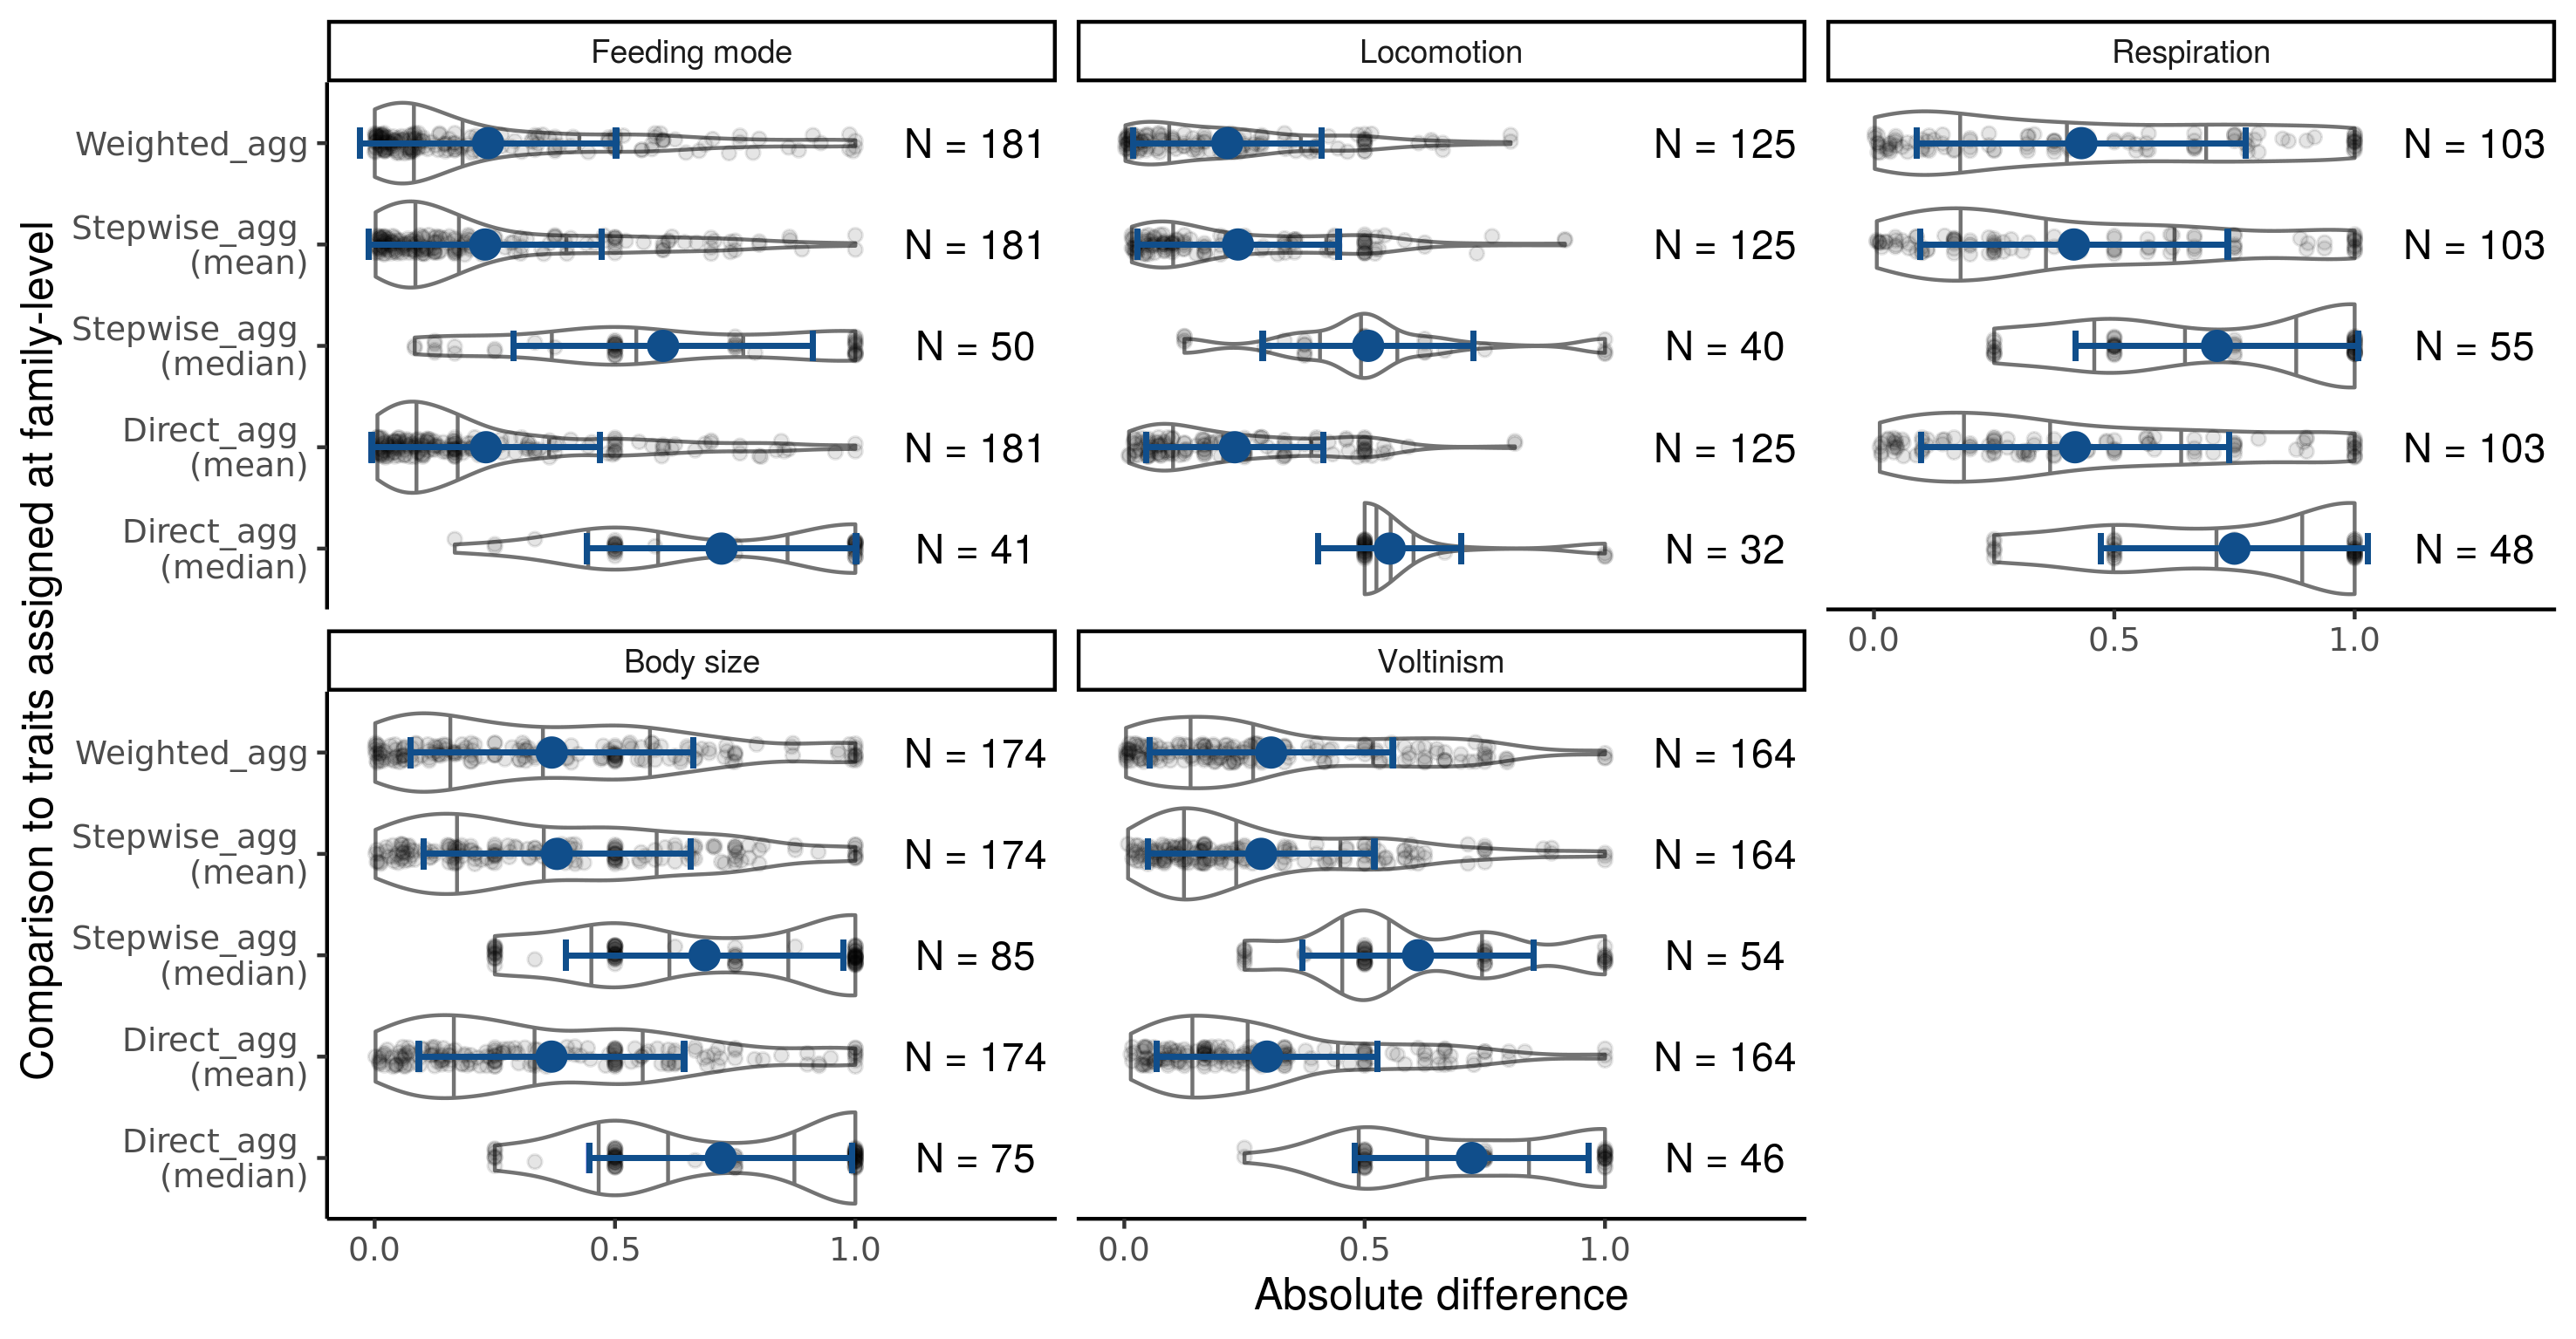
\includegraphics[width=15cm, height=12cm]{Deviances_trait_agg_pyne.png}
    \caption{Cases (factor combination of investigated families and traits) where differences occurred between aggregated traits and expert assigned traits at family level for the North American dataset. Violin plots - mirrored density plots - show the density of the absolute trait affinity differences for the grouping features locomotion, respiration, and body size. For more details see Figure \ref{fig:diff_aggr_traits_combined}.}
    \label{fig:diff_aggr_traits_pyne}
  \end{figure}


\subsubsection*{Comparison of aggregation methods with varying taxonomic hierarchies and trait variability}

\begin{figure}[H]
    \centering
    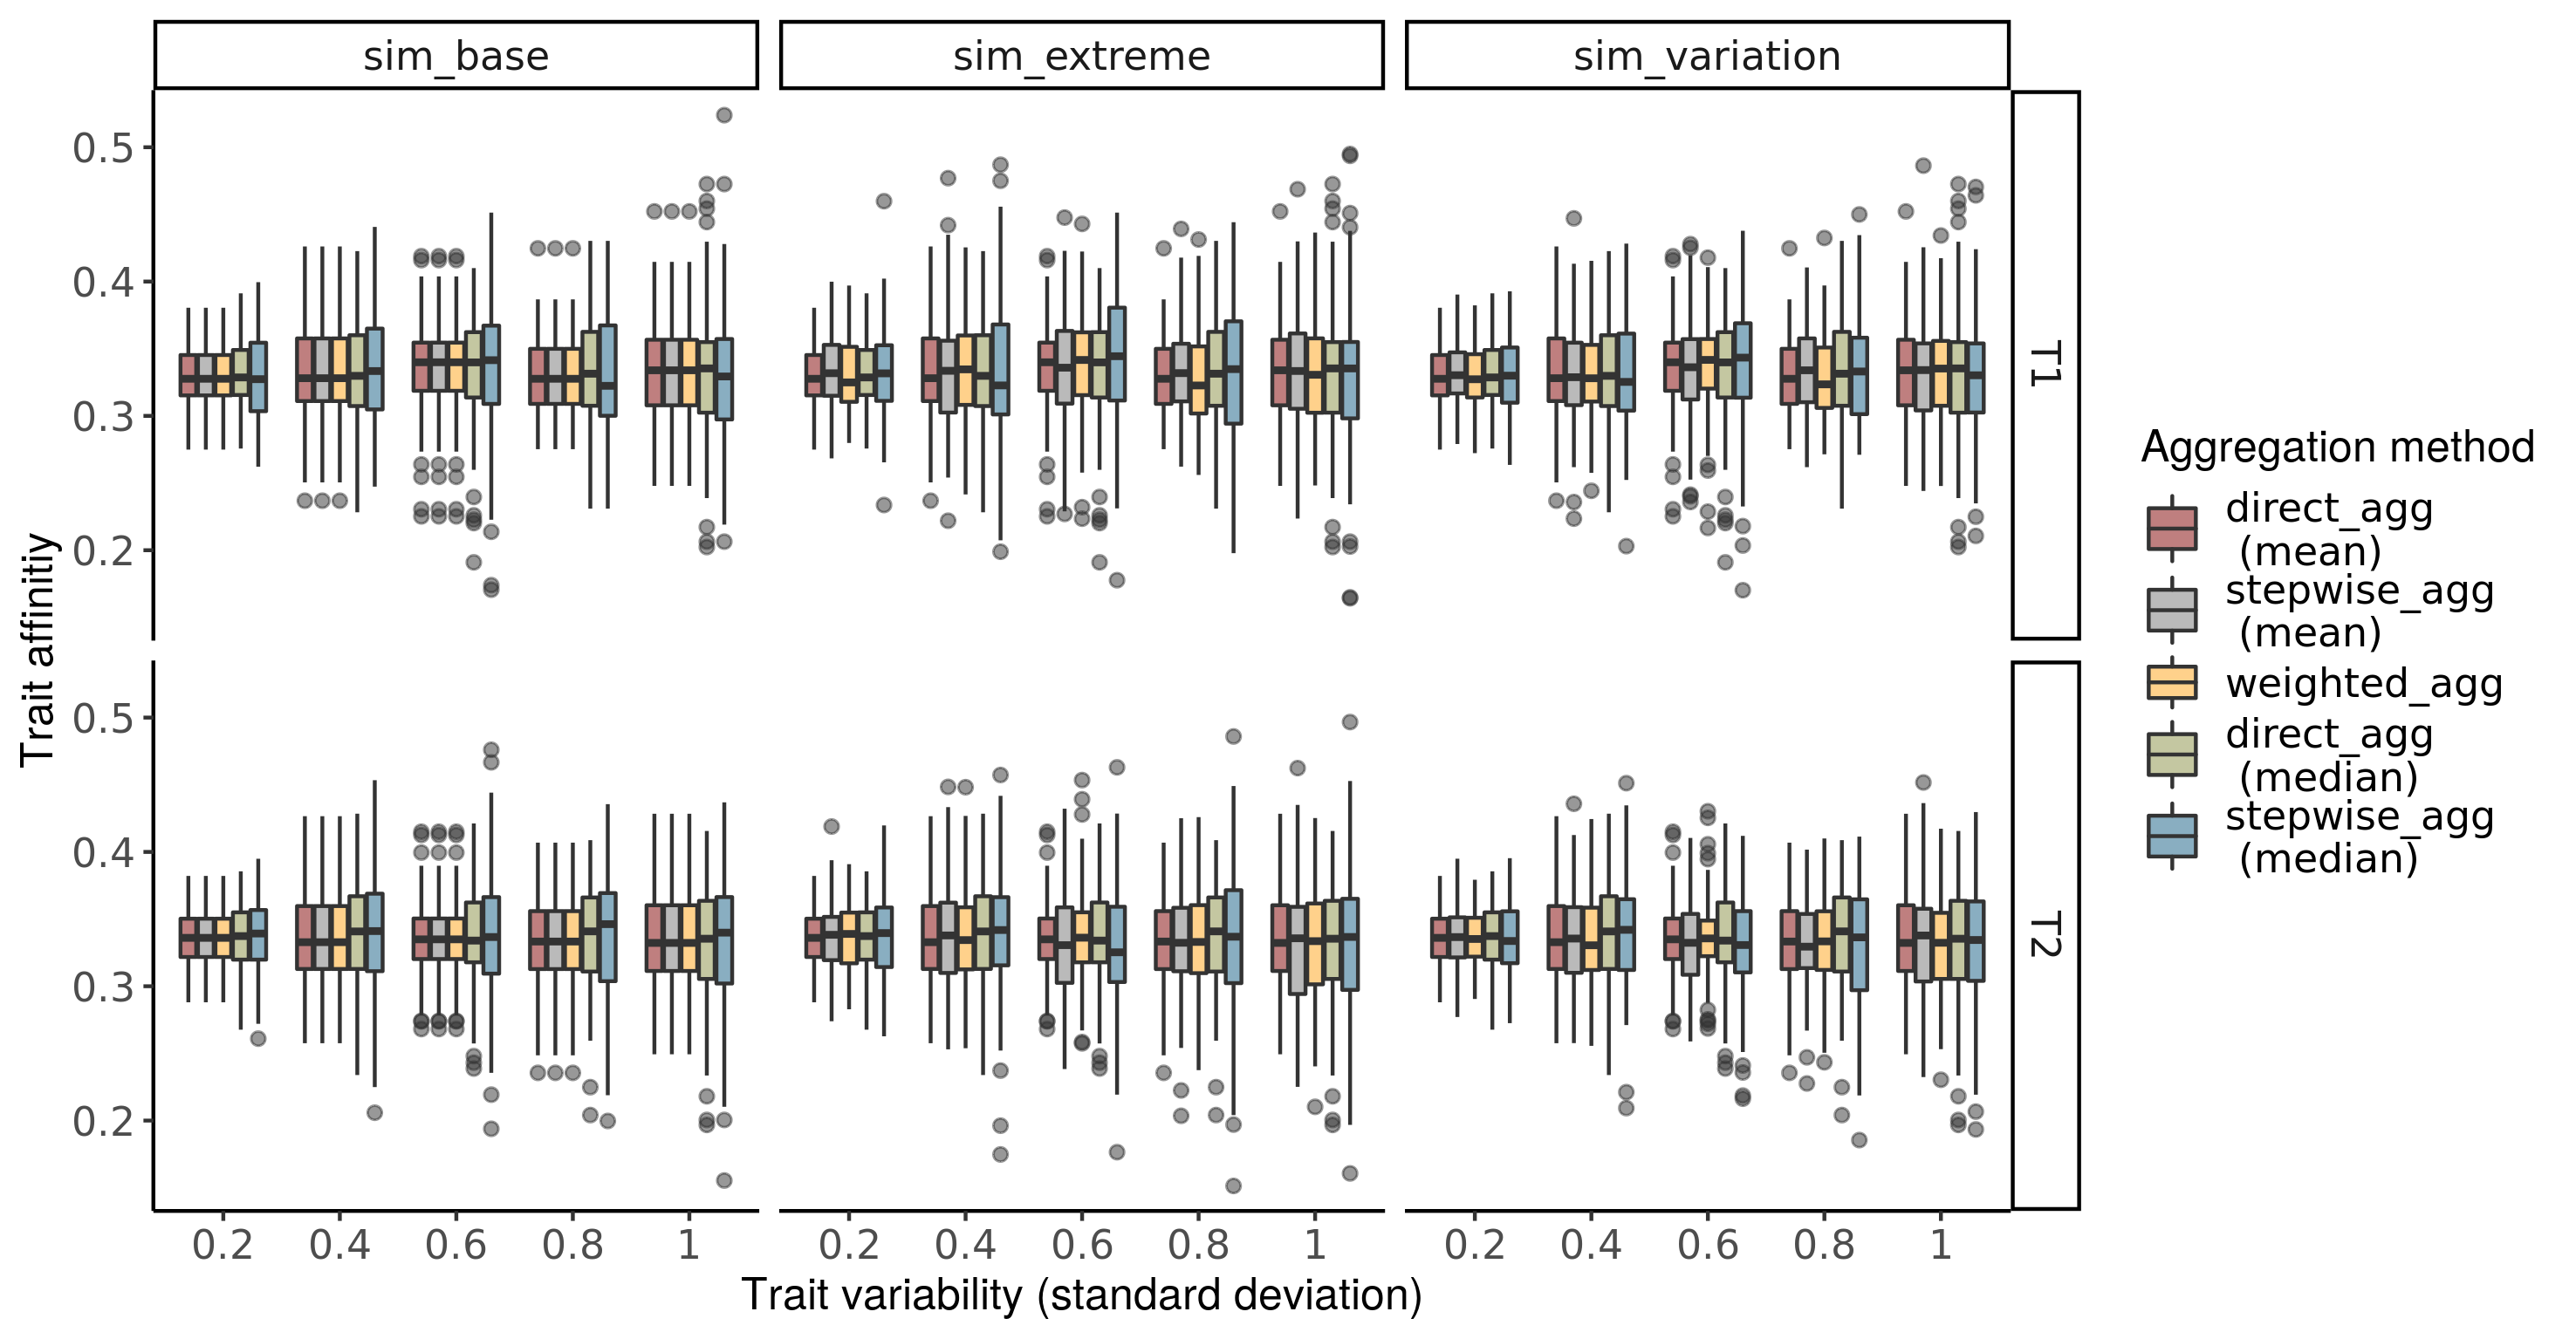
\includegraphics[width=16.5cm, height=10cm]{Overview_sim_results_T2_T3.png}
    \caption{Ranges of aggregated trait affinities for the three examples of taxonomic hierarchies and simulated levels of trait variability. Shown are the results for the simulated traits T2 and T3. Boxplots depict results for 100 replicated simulations of each trait aggregation method. Trait aggregation methods are in order of least to greatest produced ranges to improve visual inspection. For more details see Figure \ref{fig:overview_sim_results}.}
    \label{fig:overview_sim_results_T2_T3}
  \end{figure}

\subsubsection*{Taxonomic hierarchy in the trait datasets used for comparisons with assigned traits at family level}
\label{sec:taxonomic_hierarchy}

\begin{figure}[H]
    \centering
    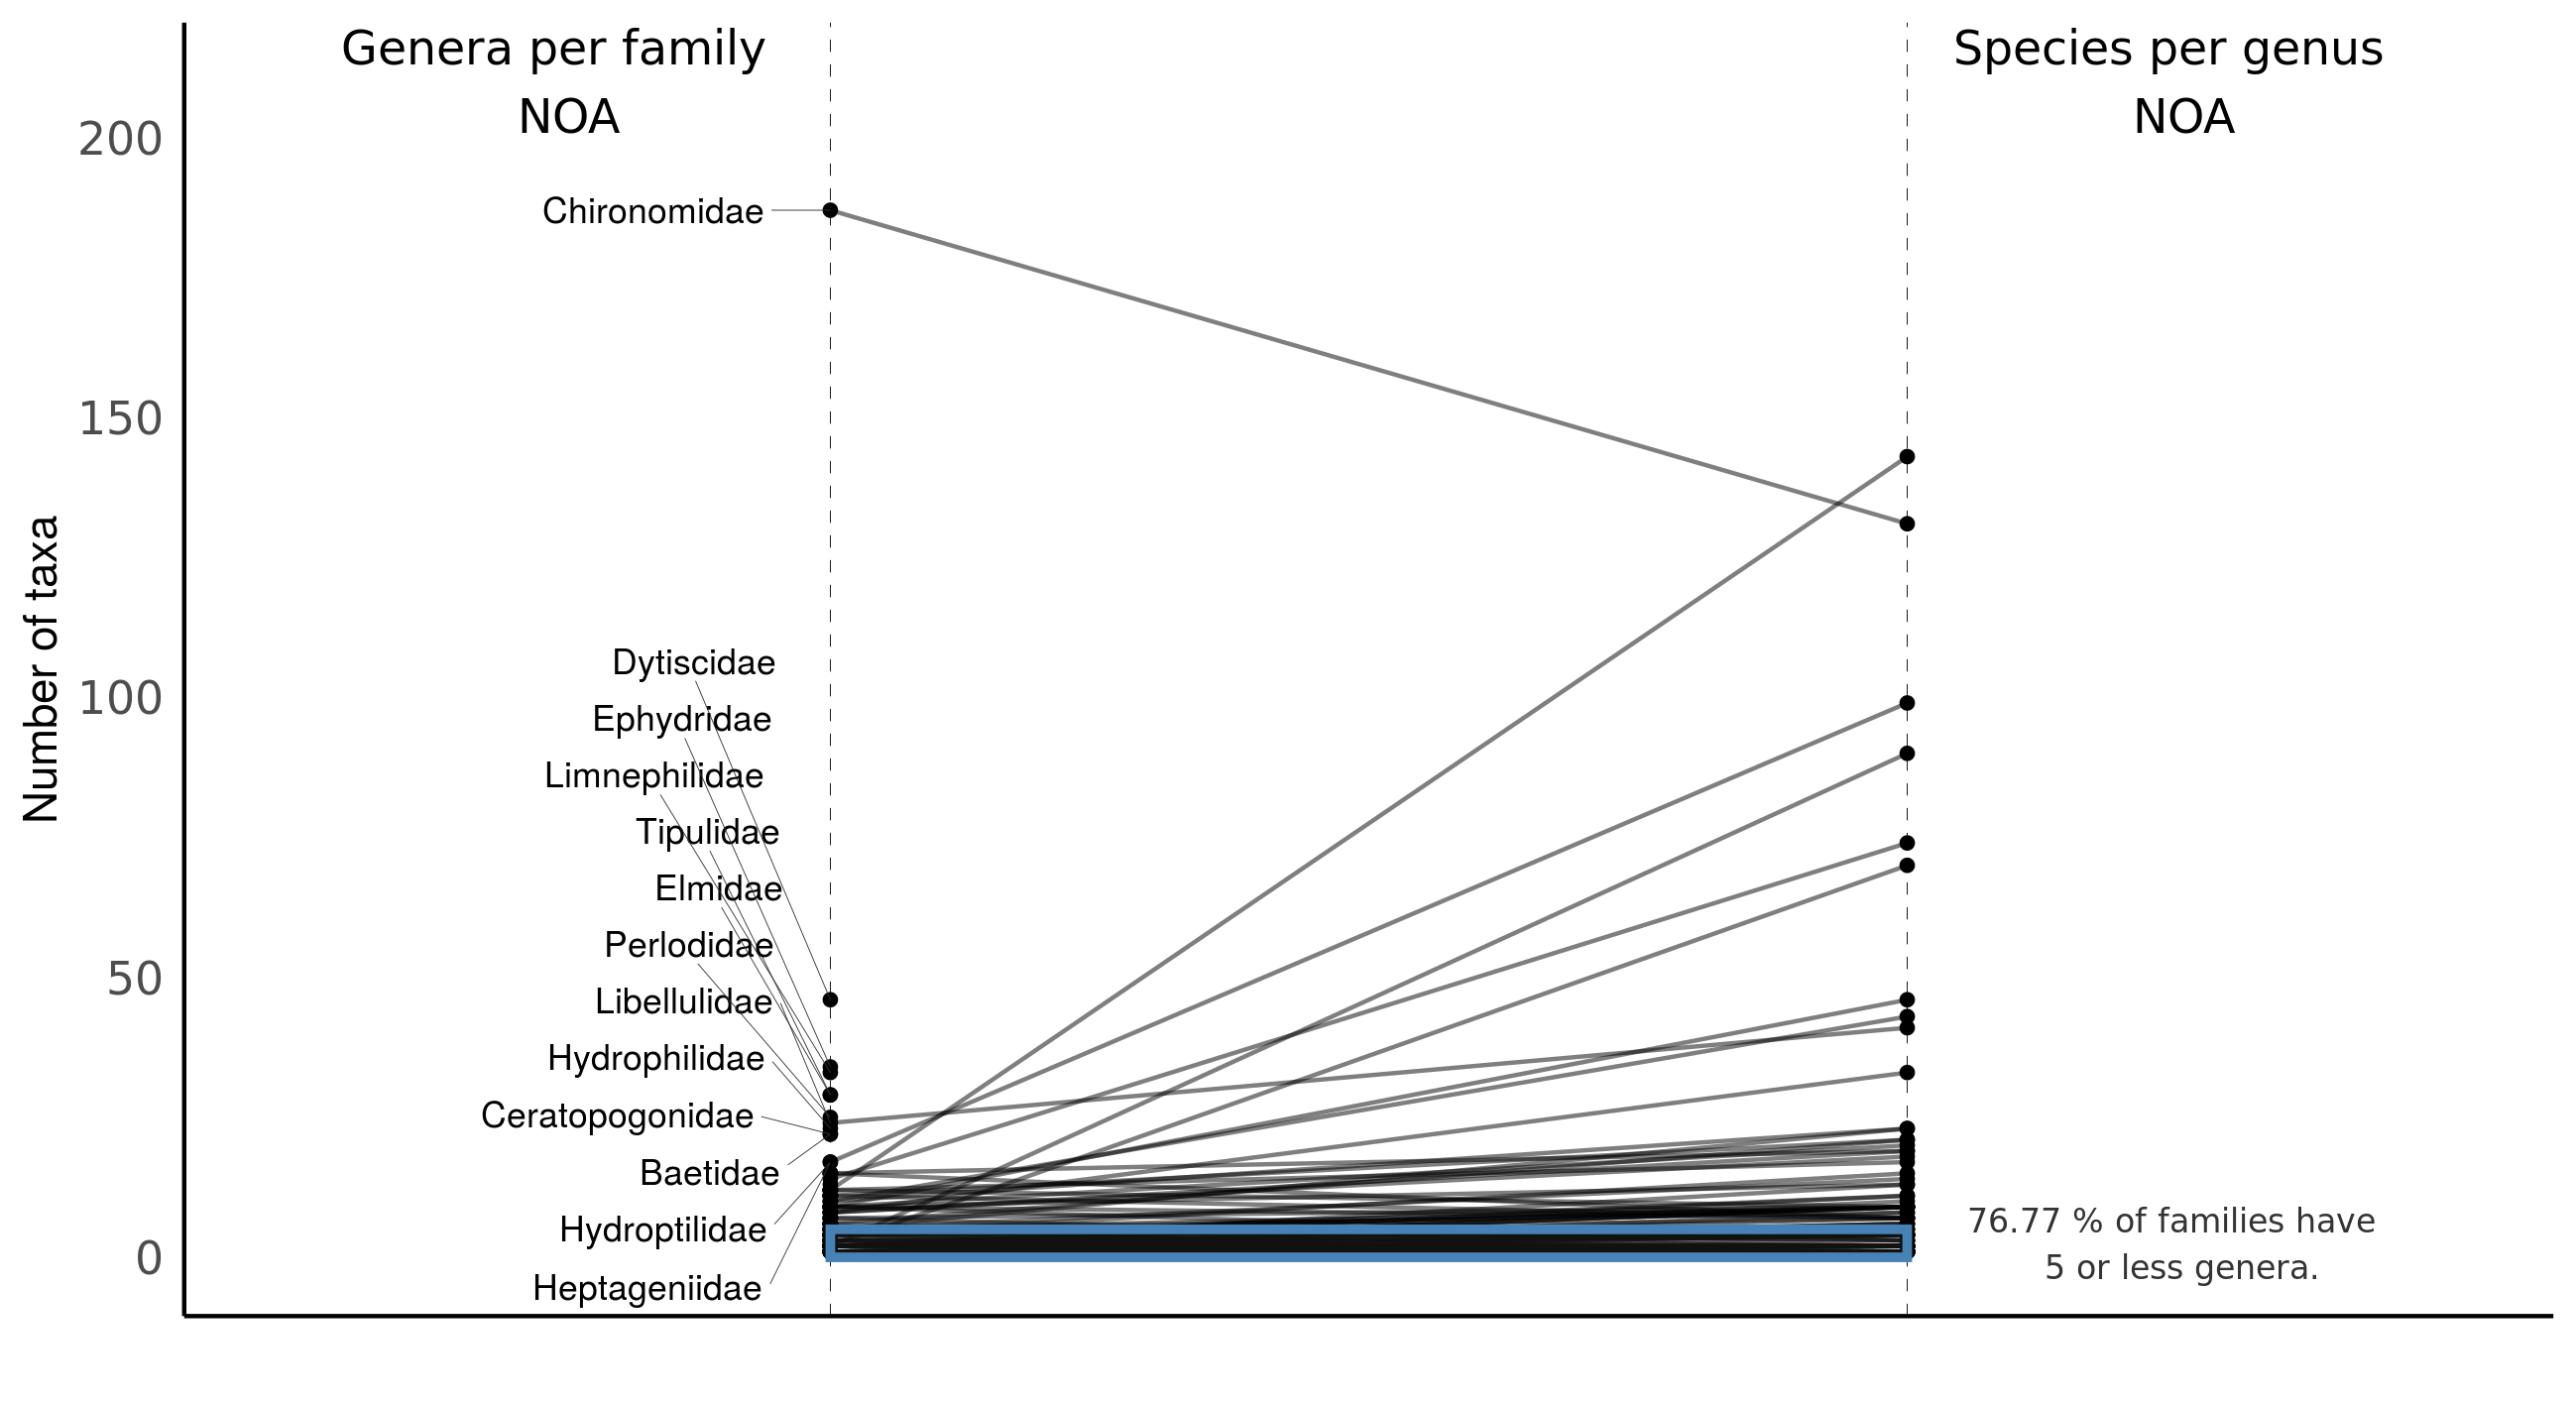
\includegraphics[width=16.5cm, height=10cm]{taxonomic_hierarchy_NOA.png}
    \caption{Number of genera per family and species per genus for those families of the North American trait dataset that have been compared with assigned traits at family level. For better visual display only families with more than 15 genera are displayed.}
    \label{fig:tax_hierarchy_NOA}
\end{figure}

\begin{figure}[H]
    \centering
    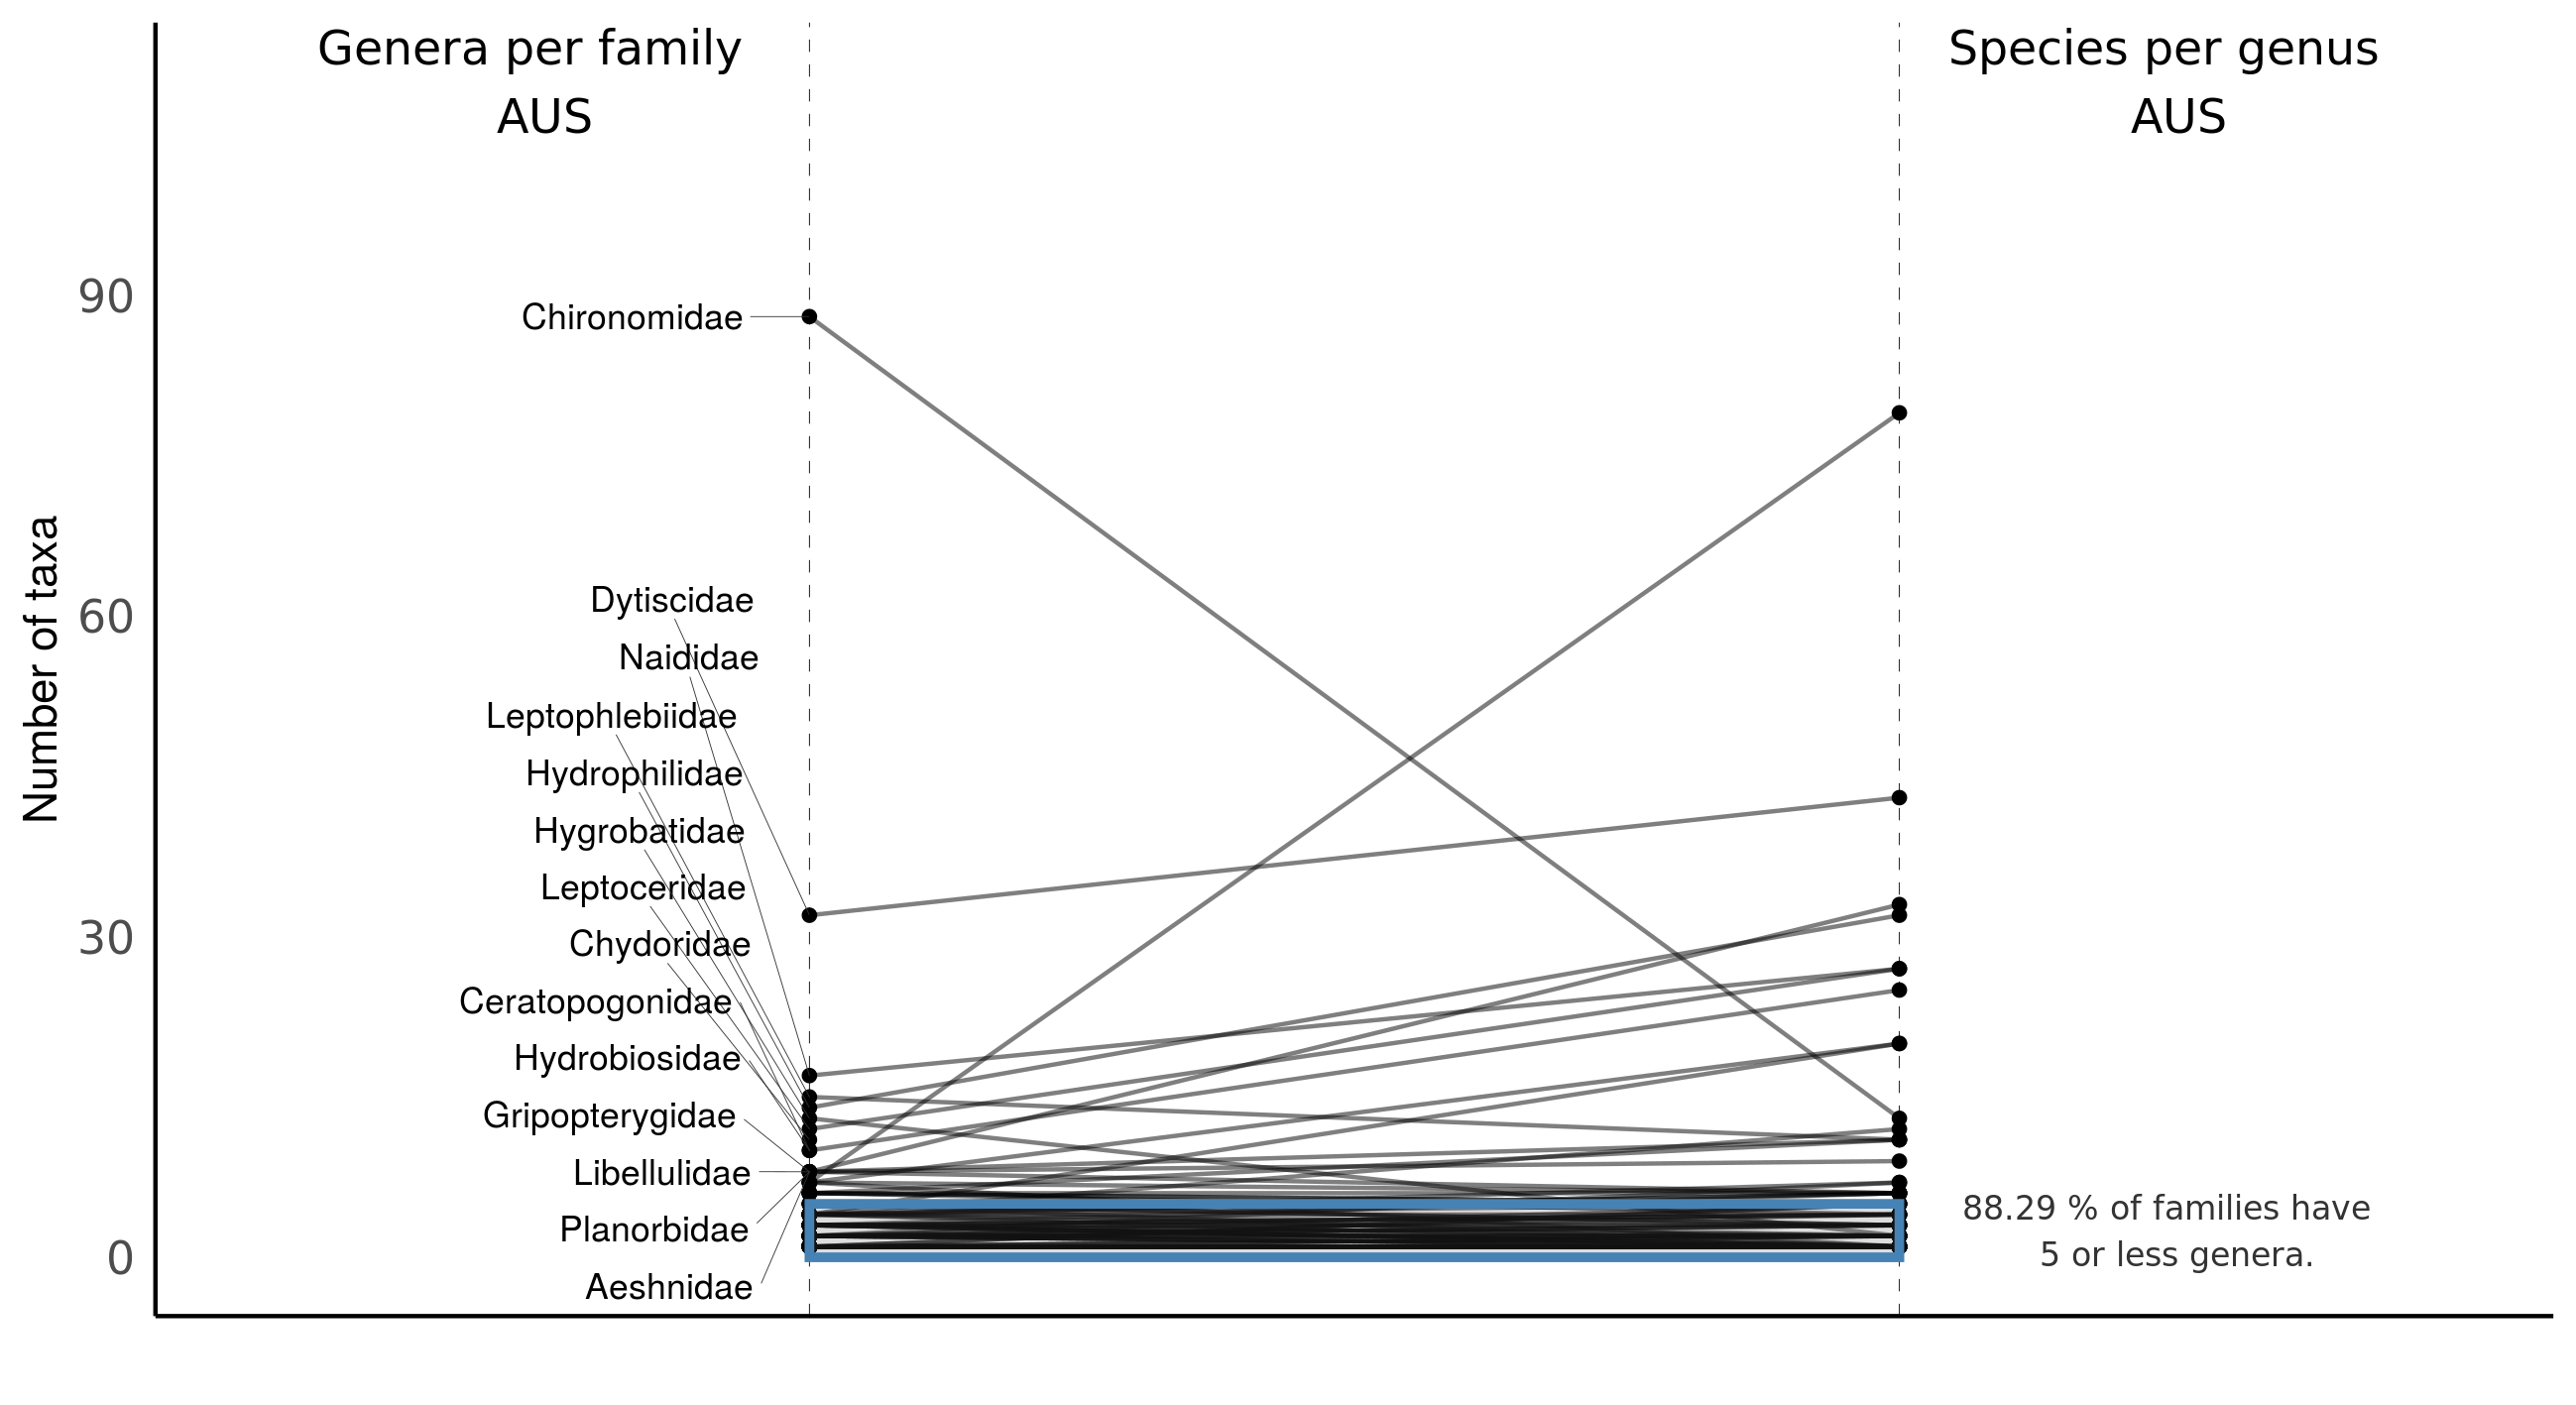
\includegraphics[width=16.5cm, height=10cm]{taxonomic_hierarchy_AUS.png}
    \caption{Number of genera per family and species per genus for the Australian trait dataset. For better visual display only families with more than 7 genera are displayed.}
    \label{fig:tax_hierarchy_AUS}
\end{figure}

\newpage

\subsection*{Effects of harmonisation and trait aggregation on inferences regarding trait-environment relationships}

\begin{table}[ht]
    \centering
    \caption{Mean, median and standard deviation of the affinities of traits that were responsive to the salinity gradient in the original study but not in the re-analysis using the harmonised European trait dataset.} 
    \label{tab:SI_resp_traits_summary_stats}
    \begin{tabular}{l|l|c|c|c|c}
    \toprule[.1em]
    Type & Trait & Mean & Median & SD & Responsive? \\ 
    \toprule[.1em]
    Stepw\_median & Shredder & 0.20 & 0.14 & 0.25 & No \\ 
      Stepw\_mean & Shredder & 0.18 & 0.12 & 0.22 & No\\ 
      Direct\_median & Shredder & 0.21 & 0.14 & 0.25 & No\\ 
      Direct\_mean & Shredder & 0.19 & 0.14 & 0.22 & No\\ 
      Weighted & Shredder & 0.19 & 0.14 & 0.22 & No \\ 
      Harmonised; not\_aggregated & Shredder & 0.18 & 0.12 & 0.24 & No \\ 
      Original & Shredder & 0.25 & 0.14 & 0.32 & Yes\\ 
      \midrule
      Stepw\_median & Gills & 0.30 & 0.27 & 0.32 & Yes\\ 
      Stepw\_mean & Gills & 0.29 & 0.22 & 0.32 & Yes\\ 
      Direct\_median & Gills & 0.30 & 0.30 & 0.32 & Yes\\ 
      Direct\_mean & Gills & 0.30 & 0.30 & 0.32 & Yes\\ 
      Weighted & Gills & 0.30 & 0.30 & 0.32 & Yes\\ 
      Harmonised; not\_aggregated & Gills & 0.30 & 0.25 & 0.32 & No \\ 
      Original & Gills & 0.28 & 0.00 & 0.33 & Yes \\ 
      \midrule
      Stepw\_median & Short life cycle & 0.64 & 0.75 & 0.39 & No \\ 
      Stepw\_mean & Short life cycle & 0.64 & 0.79 & 0.39 & No \\ 
      Direct\_median & Short life cycle & 0.67 & 0.75 & 0.37 & Yes \\ 
      Direct\_mean & Short life cycle & 0.67 & 0.79 & 0.38 & Yes \\ 
      Weighted & Short life cycle & 0.67 & 0.79 & 0.38 & Yes\\ 
      Harmonised; not\_aggregated & Short life cycle & 0.64 & 0.75 & 0.40 & Yes \\ 
      Original & Short life cycle & 0.64 & 0.75 & 0.40 & Yes \\ 
      \midrule
      Stepw\_median & Long life cylce & 0.36 & 0.25 & 0.39 & No \\ 
      Stepw\_mean & Long life cylce & 0.36 & 0.21 & 0.39 & No \\
      Direct\_median & Long life cylce & 0.33 & 0.25 & 0.37 & Yes\\ 
      Direct\_mean & Long life cylce & 0.33 & 0.21 & 0.38 & Yes \\ 
      Weighted & Long life cylce & 0.33 & 0.21 & 0.38 & Yes \\ 
      Harmonised; not\_aggregated & Long life cylce & 0.36 & 0.25 & 0.40 & Yes \\ 
      Original & Long life cylce & 0.36 & 0.25 & 0.40 & Yes\\ 
    \bottomrule
    \end{tabular}
\end{table}

\begin{figure}[ht]
    \centering
    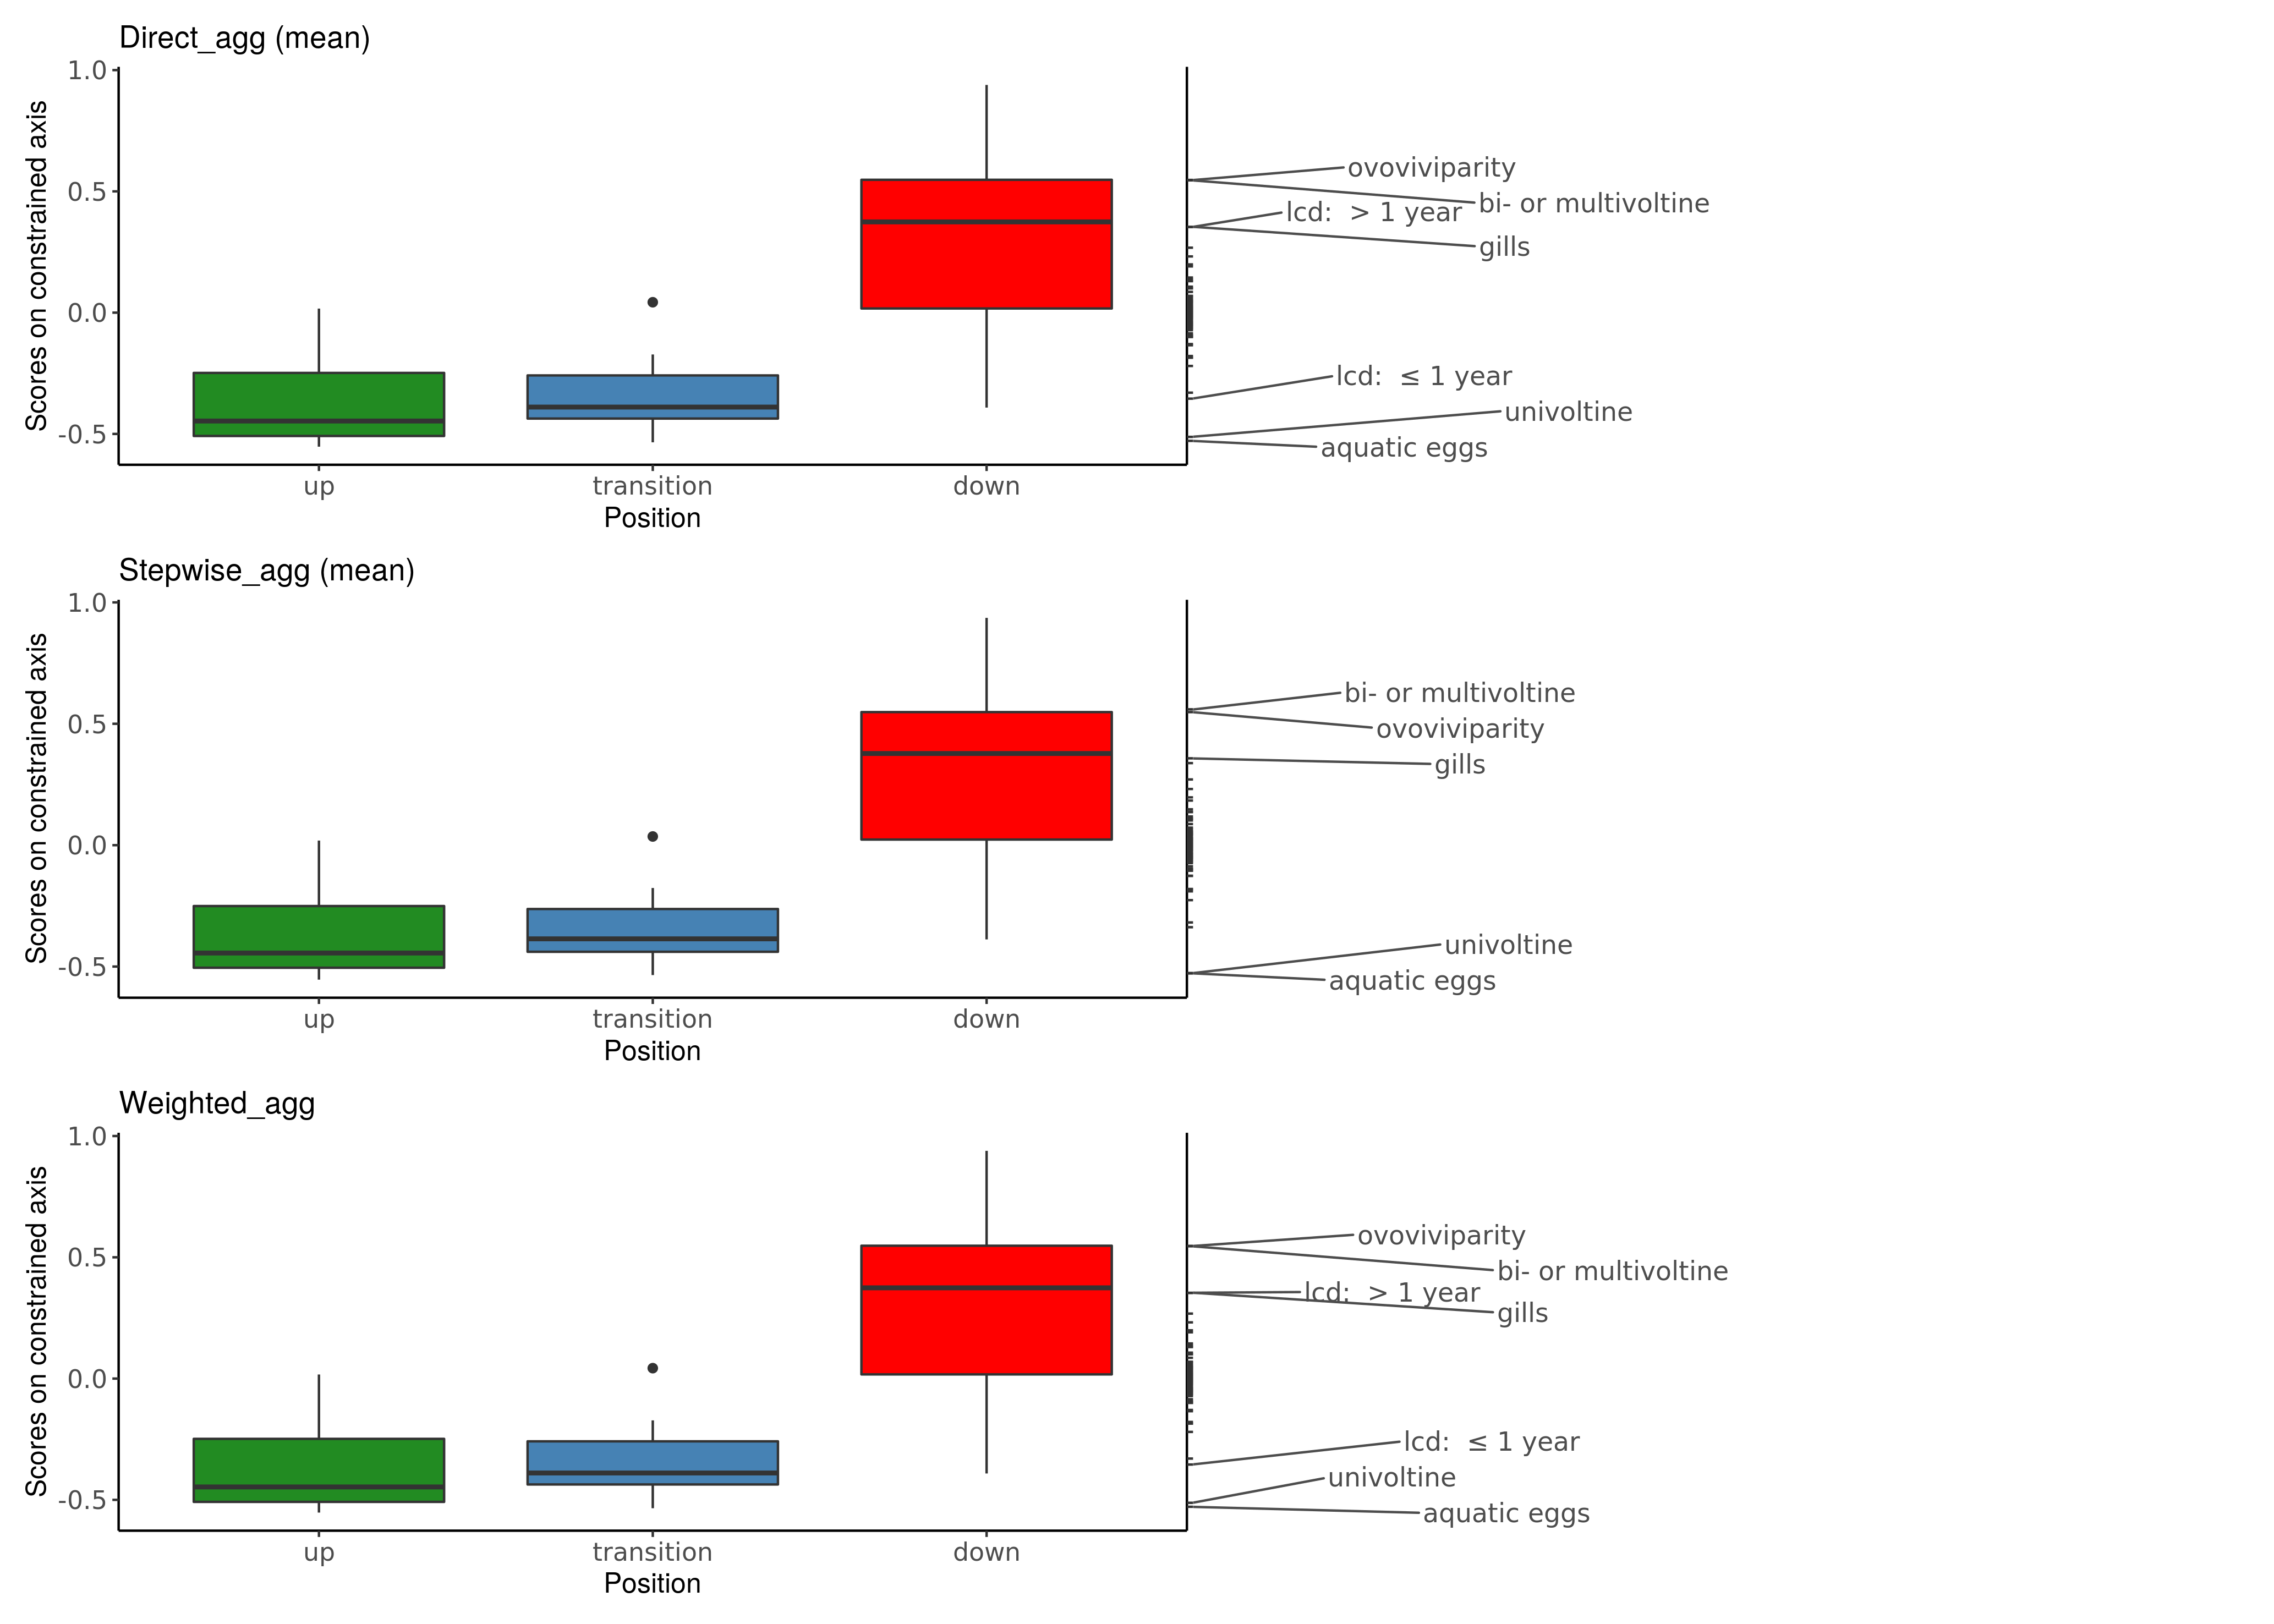
\includegraphics[width=18.5cm, height=16cm]{boxplot_scores_combined_REMAIN_SI.png}
    \caption{RDA of traits constrained by electric conductivity for the data aggregated with \textit{direct\_agg \textsubscript{mean}}, \textit{stepwise\_agg \textsubscript{mean}}, and \textit{weighted\_agg}. Shown are boxplots of the site scores along the conductivity axis. The rug on the right side of each plot indicates species scores of the traits on the conductivity axis. For more details see Figure \ref{fig:boxplot_scores_on_constrained_axis}. Abbreviations: lcd, life cycle duration; nr.cy, potential number of cycles per year.}
    \label{fig:boxplots_scores_on_constrained_axis_REMAIN}
\end{figure}


\end{document}